% Copyright 2021 Joel Feldman, Andrew Rechnitzer and Elyse Yeager, except where noted.
% This work is licensed under a Creative Commons Attribution-NonCommercial-ShareAlike 4.0 International License.
% https://creativecommons.org/licenses/by-nc-sa/4.0/

\section{1.3 The Limit of a Function}
\begin{frame}{ Table of Contents}
\mapofcontentsA{\ac}
 \end{frame}
 %--------
%----------------------------------------------------------------------------------------
%----------------------------------------------------------------------------------------

\begin{frame}
\begin{block}{Notation~\eref{text}{ntn_1_3_1} and Definition~\eref{text}{def_1_3_1}}
\[\lim_{x \to a}~ f(x)=L\]
\alert{where $a$ and $L$ are real numbers}\\
We read the above as ``the limit as $x$ goes to $a$ of $f(x)$ is $L$."

Its meaning is: as $x$ gets very close to (but not equal to) $a$, $f(x)$ gets very close to $L$.
\end{block}
\end{frame}
%----------------------------------------------------------------------------------------
\begin{frame}{Finding Slopes of Tangent Lines}

 We NEED limits to find slopes of tangent lines.\hfill
 
\includegraphics[width=1cm]{Clipart/dogeyes}
\index{

\includegraphics[height=5mm]{Clipart/dogeyes} \href{https://creativecommons.org/licenses/by/3.0/}{`Dog'} by 
\href{https://thenounproject.com/iconsfromrussia/}{Vladimir Belochkin} is licensed under \CCBYthree~ (accessed 17 June 2021)}
\note<1>{Students often forget this: remind them that if we try to take an interval of length 0, it causes us to divide by zero.

 This is also a nice example to hearken back to later when someone asks why zero divided by zero isn't just 1.}

\begin{center}
\begin{tikzpicture}
\draw[thick] plot[domain=0.25:1.75](2*\x,{2-2*\x*\x+4*\x});
\draw (1,3.5) node[vertex]{};
\foreach \t in {2,...,7}{
	\onslide<\t>{
		\MULTIPLY{\t}{2}{\x}
		\draw ({2-0.1*(\x-5)},{4-(\x-5)*(\x-5)/200}) node[C2, vertex]{};}}
\end{tikzpicture}
\end{center}\StatusBar{2}{7}
\note<3>{``This is fine, this is fine, this is still fine..." (during animation)}
\vfill
\onslide<2->{Slope of secant line: $\dfrac{\Delta y}{\Delta x}$, \textcolor{C3}{$\Delta x \neq 0$}.\\}
\onslide<7->{Slope of tangent line: \textcolor{C3}{can't do the same way}.}
\vfill
\note<8>{Here I'm intentionally mixing ``slope of tangent line" and ``instantaneous rate of change" as an opportunity to remind students verbally that they're the same thing.

Verbally describe during animation how we're taking an average RoC over smaller and smaller intervals, approximating a rate of change. Since we can't actually plug in only one point, we take a limit.

We just showed a limit at x=5; this one only differs because we're using a parameter now. Pause is there before the formula so you can write it out and explain bit by bit.
}
\onslide<8->{\textcolor{M2}{If the position of an object at time $t$ is given by $s(t)$, then its instantaneous velocity is given by}\onslide<9->{ \[\ds\lim_{h \to 0}~\dfrac{s(t+h)-s(t)}{h}\]}}


\end{frame} 
%-------- %--------
\note{So, limits are going to be an important part of our lives for the next little while. Let's think about a few of them.}
%----------------------------------------------------------------------------------------
\begin{frame}[t]{Evaluating Limits}

\begin{center}Let~ $f(x)=\displaystyle\frac{x^3+x^2-x-1}{x-1}$.\end{center} We want to evaluate $\displaystyle\lim_{x \rightarrow 1}~ f(x)$.
\only<beamer>{\vfill

\only<2-3>{What is $f(1)$?} \only<3>{\textcolor{C2}{DNE} (can't divide by zero)}
\note<4>{Can pull up a spreadsheet program and make the table in real time, for theatrics}
\only<4->{ Use the tables below to guess
$\displaystyle\lim_{x \rightarrow 1}~ f(x) $
\begin{center}
\begin{tabular}{l|l}
$x$&$f(x)$\\
\hline
0.9 &3.61\\
0.99&3.9601\\
0.999&3.99600\\
0.9999&3.99960
\end{tabular}
\qquad
\begin{tabular}{l|l}
$x$&$f(x)$\\
\hline
1.1&4.41\\
1.01&4.0401\\
1.001&4.00400\\
1.0001&4.00040
\end{tabular}
\end{center}}

\onslide<5->{\vfill\[\textcolor{answercolor}{\boxed{\lim_{x \to 1}~f(x)=4}}\]}

\only<2>{\QuestionBar{1}{4} \AnswerYes}
\only<3>{\AnswerBar{1}{4}}
\only<4>{\QuestionBar{2}{4}\AnswerYes}
\only<5>{\AnswerBar{2}{4}}}

\unote{Example~\eref{text}{eg_1_3_2}}
\end{frame}
 %--------

%----------------------------------------------------------------------------------------
\begin{frame}[t]{One-Sided Limits}

\begin{center}
\begin{tikzpicture}[scale=0.7]
\draw (7,2)node[right,fill=white,inner sep=0]{\small $f(x)=\left\{
\begin{array}{rl}
x&\mbox{ if }x<3 \\
1&\mbox{ if }x=3\\
x-1&\mbox{ if }x>3
\end{array}
\right.$
};
\myaxis{x}{0}{6.2}{}{0}{5.2}
\draw[dotted, thin] (0,0) grid (6,5);
   \draw[scale=1,domain=0:2.9,smooth,variable=\x,C2, ultra thick] plot ({\x},{\x});
   \draw[scale=1,domain=3.1:6,smooth,variable=\x,C2, ultra thick] plot ({\x},{\x-1})
   node[right] {$y=f(x)$};
      	
\draw (3,3) node[C2, opendot]{};
\draw (3,2) node[C2, opendot]{};
\draw (3,1) node[C2, vertex]{};

\foreach \x in {0,...,6}{
	\draw (\x,0) node[below]{$\x$};}
\foreach \x in {0,...,5}{
	\draw (0,\x) node[left]{$\x$};}
\end{tikzpicture}
\end{center}

\only<-2>{What do you think $\displaystyle\lim_{x \rightarrow 3}~ f(x)$ should be?}
\only<beamer>{\qquad\onslide<2>{\textcolor{answercolor}{DNE}}

\onslide<3->{Evaluate: 
$
\underbrace{\displaystyle\lim_{x \rightarrow 3^-}~ f(x)}_{\mbox{from the left}}\onslide<4->{\textcolor{answercolor}{=3}} \qquad 
\underbrace{\displaystyle\lim_{x \rightarrow 3^+}~ f(x)}_{\mbox{from the right}}\onslide<5->{\textcolor{answercolor}{=2}}
$}
\only<1-4>{\AnswerYes}
\only<1>{\QuestionBar{3}{4}}
\only<2>{\AnswerBar{3}{4}}
\only<3>{\QuestionBar{4}{4}}
\only<4-5>{\AnswerBar{4}{4}}
}
\note<4>{\small What the limit should be can generate some good class discussions. Can ask to raise hands: Who thinks it's 1/2/3/more than one / none, etc.

That motivates the need for left and right limits. Explain verbally for this slide.

It can be helpful to remind students that we needed limits before precisely because there was something fishy going on at a point. So if we were to say that the limit were equal to the value, it wouldn't capture the fishy behaviour. You can also ask -- how would you want to describe the behaviour of the function? This motivates our ideas of limits, for students whose instinct is often that the value of the function should equal the limit because that's somehow the important value.}
\unote{Example~\eref{text}{eg_1_3_3}}
\end{frame}
 %--------

\begin{frame}
\begin{block}{Definition~\eref{text}{def informal onesided limits}}
The limit as $x$ goes to $a$ \textbf{ from the left} of $f(x)$ is written
\[\lim_{x \to a^-}~ f(x)\]
We only consider values of $x$ that are \alert{less than} $a$.

\vspace{1em}
The limit as $x$ goes to $a$ \textbf{ from the right} of $f(x)$ is written
\[\lim_{x \to a^+}~ f(x)\]
We only consider values of $x$  \alert{greater than} $a$.
\end{block}

\end{frame}
 %--------
\begin{frame}
\begin{block}{Theorem~\eref{text}{thm_1_3_1}}
In order for $\ds\lim_{x \to a}~ f(x)$ to exist, both one-sided limits must exist and be equal.
\end{block}\vfill
\begin{tikzpicture}[scale=0.8]
\myaxis{x}{0}{6.2}{y}{0}{5.2}
\draw[step=1cm, ultra thin] (0,0) grid (6,5);
   \draw[scale=1,domain=0:2.9,smooth,variable=\x,C2, ultra thick] plot ({\x},{\x});
   \draw[scale=1,domain=3.1:6,smooth,variable=\x,C2, ultra thick] plot ({\x},{\x-1})
   node[right] {$y=f(x)$};
      	
\draw (3,3) node[C2, opendot]{};
\draw (3,2) node[C2, opendot]{};
\draw (3,1) node[C2, vertex]{};

\foreach \x in {0,...,6}{
	\draw (\x,0) node[below]{$\x$};}
\foreach \x in {0,...,5}{
	\draw (0,\x) node[left]{$\x$};}
\end{tikzpicture}
\end{frame}
 %--------
%----------------------------------------------------------------------------------------
\begin{frame}[t]
\AnswerSpace\only<2>{\AnswerYes}
\only<1>{Consider the function $f(x)=\displaystyle\frac{1}{(x-1)^2}$.}
\only<1>{For what value(s) of $x$ is $f(x)$ \alert{not} defined?\\[1em]\AnswerNo}

\only<beamer>{
\only<2->{Based on the graph below, what would you like to write for:
\[\lim_{x \rightarrow 1} ~f(x)=\onslide<3-|handout:0>{\alert{\infty}}\] }}


\only<beamer>{
\vspace{-1em}
\begin{tikzpicture}[yscale=.8]
\myaxis{x}{2}{6.2}{}{0}{6.2}
\draw[scale=1,domain=-2:0.591,smooth,variable=\x,C2, ultra thick] plot ({\x},{1/((\x-1)*(\x-1))});
\draw[scale=1,domain=1.409:6,smooth,variable=\x,C2, ultra thick] plot ({\x},{1/((\x-1)*(\x-1))});
\draw[C2] (4.5,1)   node[fill=white,inner sep=0] {$f(x) = \frac{1}{(x-1)^2}$};
\xcoord{1}{1}
\end{tikzpicture}}


\onslide<3|handout:0>{
\vspace{-5cm} \colorbox{white}{\parbox{\linewidth}{A subtle point: we say that this limit \alert{does not exist}. It ``does not exist" in a way that we can, nonetheless, describe.}}
}
\note<3>{It's nice to explain verbally that the distinction is only really important in their lives for parsing theorems. If something says ``if the limit exists...." then it might not apply here. It's still standard to write ``equals infinity."}
\end{frame}
%----------------------------------------------------------------------------------------

%----------------------------------------------------------------------------------------
\begin{frame}[t]{A Stranger Limit Example}
\unote{Example~\eref{text}{eg sinpix}}
\begin{center}\begin{tikzpicture}
\myaxis{x}{5}{5}{y}{1.5}{1.5}
\draw (0,0)node{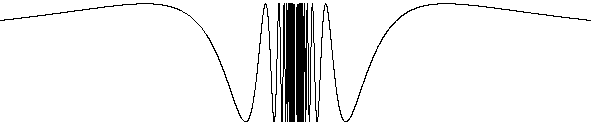
\includegraphics{fig/sin1x.pdf}};
\draw (4,1.5)node{$f(x)=\sin\left(\displaystyle\frac{1}{x}\right)$};
\end{tikzpicture}\end{center}

\begin{QuestionSet}
\SetQuestion{What is $\lim\limits_{x \to \infty}~ f(x)$ ?\AnswerYes}
\SetAnswer{What is $\lim\limits_{x \to \infty}~ f(x)$ ?\\[1mm]\textcolor{answercolor}{$\lim\limits_{x \to \infty}~ f(x) = 0$}}
\SetQuestion{What is $\lim\limits_{x \to 0}~ f(x)$ ?\AnswerYes}
\SetAnswer{What is $\lim\limits_{x \to 0}~ f(x)$ ?\\[1mm]\textcolor{answercolor}{$\lim\limits_{x \to 0}~ f(x)$  does not exist.}\vfill We can call this behaviour ``infinite wiggling."}
\SetQuestion{What is $\lim\limits_{x \to \pi}~ f(x)$ ?\AnswerYes}
\SetAnswer{What is $\lim\limits_{x \to \pi}~ f(x)$ ?\\[1mm]\textcolor{answercolor}{$\lim\limits_{x \to \pi}~ f(x) = \sin\left(\frac1\pi\right)$}}
\end{QuestionSet}
\end{frame}
%----------------------------------------------------------------------------------------
%----------------------------------------------------------------------------------------
\begin{frame}[t]{Optional: Sketching $f(x)=\sin\left(\frac1x\right)$ \only<beamer>{\hfill \hyperlink{sketchingover}{\beamerskipbutton{skip sketching}}}}
\begin{tikzpicture}
\COPY{.45}{\scx}%scale for x
\COPY{12}{\sct}%scale for theta
\COPY{4}{\ysh}%yshift
\DIVIDE{\numberPI}{2}{\halfpi}

\myaxis{\theta}{0}{8}{}{1.25}{1.25}
\draw (8.75,0)node[right]{$y=\sin\theta$};
\draw plot [domain=0:8/\scx,smooth,samples=50]({\x*\scx},{sin(\x r)});
\onslide<2->{\xcoord{\halfpi*\scx}{\frac{\pi}{2}}}


\begin{scope}[yshift=\ysh cm]
\myaxis{x}{0}{8}{}{1.25}{1.25}
\draw (8.75,0)node[right]{$y=\sin \frac1x$};
\onslide<3->{\xcoord{\sct/\halfpi}{\frac2{\pi}}}
\end{scope}

\foreach \n in {1,...,5}{
	\MULTIPLY{\n}{3}{\s}%three overlays for each piece: thetacoord highlight, x coords, x graph
	\SUBTRACT{\s}{1}{\sa} %on this slide, show the sintheta
	\ADD{\sa}{1}{\sb} %on this slide, find corresponding x- coordinates
	\ADD{\sa}{2}{\sc} %on this slide, show sin(1/x)
	
	\MULTIPLY{\n}{2}{\a}
	\ADD{\a}{1}{\b}
	\SUBTRACT{\a}{1}{\a}
	\MULTIPLY{\a}{\numberPI}{\api}
	\MULTIPLY{\b}{\numberPI}{\bpi}
	\DIVIDE{\bpi}{2}{\bpih}%b pi / 2 , "b*pi half"
	\onslide<\sa->{
		\draw[line width=4pt, C\n, opacity=0.5] plot[domain=\api/2:\bpi/2,xscale=\scx](\x,{sin(\x r)});
		\xcoord{\bpih*\scx}{\frac{\b\pi}{2}}
		}
	\iftoggle{printsolutions}{
	\begin{scope}[yshift=\ysh cm]
	\onslide<\sb->{
		\ifodd \n
		\draw(\sct/\bpih,0.2)--+(0,-.4) node[below,yshift=-7mm]{\footnotesize \alert<\sb|handout:0>{$\frac{2}{\b\pi}$}};
		\else
		\draw(\sct/\bpih,-0.2)--+(0,.4) node[above,yshift=7mm]{\footnotesize \alert<\sb|handout:0>{$\frac{2}{\b\pi}$}};
		\fi
		}
	\onslide<\sc->{
		\draw[C\n, line width=2pt] plot[domain=2/pi/\b:2/pi/\a,xscale=\sct,samples=100](\x,{sin(1/\x r)});}
	\end{scope}
		}{}}
\end{tikzpicture}
\StatusBar{1}{16}

\end{frame}
%----------------------------------------------------------------------------------------
%----------------------------------------------------------------------------------------
\begin{frame}{Limits and the Natural Logarithm}\label<1|handout:1>{sketchingover}%skip here if you don't want to go over sketching sin(1/x)
\AnswerSpace
\begin{QuestionSet}
\SetQuestion{Where is $f(x)$ defined, and where is it not defined? \AnswerNo}
\SetQuestion{What can you say about the limit of $f(x)$ near 0? \AnswerYes}
\SetAnswer{What can you say about the limit of $f(x)$ near 0?  \textcolor{answercolor}{$\displaystyle\lim_{x \rightarrow 0^+} \log (x)=-\infty$}}
\end{QuestionSet}


\begin{center}
\begin{tikzpicture}[scale=0.8]
\myaxis{x}{2.2}{8.2}{y}{4.2}{3.2}
\draw[scale=1,domain=0.015:8,smooth,variable=\x,C2, ultra thick] plot[samples=100] ({\x},{ln(\x)});
  
\foreach \x in {-4, -2, 2}{\ycoord{\x}{\x}}
\foreach \x in {-2,2,4,6}{\xcoord{\x}{\x}}
	
\draw[C2] (5,2.6)node[fill=white]{$f(x)=\log x$};
\end{tikzpicture}
\end{center}
\note<2>{We put an example between this and the last limit going to infinite intentionally, to allow students' short-term memory to clear a little. Now when we ask whether this limit exists, we get to reinforce rather than just reiterate. 

The question is also asked a little vaguely, since we \textbf{can't} say $\lim\limits_{x \to 0} = - \infty$. You can ask students to describe the behaviour to their neighbours, and prime the pump a little with a reminder about one-sided limits. Once the "limit going to infinity" business is a little clearer in students' minds, we can add this subtlety: that some kinds of limits don't exist in ways we don't have convenient notation for. }
\end{frame}
%----------------------------------------------------------------------------------------
\mode<beamer>{
\begin{frame}
Section 1.3 Review
\end{frame}}
%------------------------------------------------------------------
\begin{frame}[t]
\only<1>{\AnswerNo}
\begin{multicols}{2}
$\displaystyle f(x)=\left\{\begin{array}{ll}x^2 & x \neq 1 \\ 2& x=1 \end{array}\right.$\\[2em]


\begin{tikzpicture}[scale=0.8]
\myaxis[thick]{x}{2.2}{2.2}{}{0}{4.2}
\draw[step=1cm,  thin,dotted] (-2,0) grid (2,4);
\foreach \x in {-2,-1,1,2}{\xcoord[fill=white]{\x}{\x}}
\foreach \x in {1,...,4}{\ycoord[fill=white,yshift=2mm]{\x}{\x}}

 \draw[scale=1,domain=-2:2,smooth,variable=\x,C2, ultra thick] plot ({\x},{\x*\x});
\draw (1,1) node[C2, opendot]{};
\draw (1,2) node[C2, vertex]{};
\end{tikzpicture}


\columnbreak

What is $\displaystyle\lim_{x \rightarrow 1}~ f(x)$?

\vspace{.5cm}
\begin{itemize}
\item[A.] $\displaystyle\lim_{x \rightarrow 1 }~ f(x)=2$\vfill
\item[B.] $\displaystyle\lim_{x \rightarrow 1 }~ f(x)=1$\vfill
\item[C.] $\displaystyle\lim_{x \rightarrow 1 }~ f(x) \mbox{ DNE}$\vfill
\item[D.] none of the above\vfill
\end{itemize}


\end{multicols}
\note{Often here students need reminding that the limit doesn't necessarily equal the function. I like to point out that we can already write $f(1)=2$ to describe what happens at that point, so there's no point to defining a limit as just another way of saying that information. The limit gives us \textit{different} information.

It's also nice to point out why the limit isn't DNE. We motivated limits with slopes of tangent lines, where we were always examining functions with some weird issue at a point. If there weren't that weird issue, we wouldn't really need limits; so it doesn't make sense for a removable discontinuity to lead to a limit not existing.}
\end{frame}
 %--------

%----------------------------------------------------------------------------------------
\begin{frame}[t]
\begin{multicols}{2}
$\displaystyle f(x)=\left\{\begin{array}{rl}4 & x \leq 0\\ x^2& x>0 \end{array}\right.$\\[2em]

\begin{tikzpicture}[scale=0.8]
\myaxis[thick]{x}{2.2}{2.2}{y}{0}{4.2}
\draw[step=1cm, thin,dotted] (-2,0) grid (2,4);
\foreach \x in {-2,-1,1,2}{\xcoord{\x}{\x}}
\foreach \x in {1,...,4}{\ycoord[fill=white,yshift=2mm]{\x}{\x}}
	
   \draw[scale=1,domain=-2:0,smooth,variable=\x,C2, ultra thick] plot ({\x},{4});
   \draw[scale=1,domain=0:2,smooth,variable=\x,C2, ultra thick] plot ({\x},{\x*\x});
      	
\draw (0,0) node[C2, opendot]{};
\draw (0,4) node[C2, vertex]{};
\end{tikzpicture}



\columnbreak


\only<1-2>{What is $\displaystyle\lim_{x \rightarrow 0 }~ f(x)$?}
\only<3-4>{What is $\displaystyle\lim_{x \rightarrow 0^+ }~ f(x)$?}
\only<5>{What is $f(0)$?}

\only<1-4>{\begin{itemize}
\item[A.] $\displaystyle\lim_{x \rightarrow 0\only<4->{^+} }~ f(x)=4$\vfill
\alert<4|handout:0>{\item[B.] $\displaystyle\lim_{x \rightarrow 0\only<4->{^+} }~ f(x)=0$}\vfill
\item[C.] $\displaystyle\lim_{x \rightarrow 0\only<4->{^+} }~ f(x)=\left\{\begin{array}{rl} 4& x \leq 0 \\ 0 & x>0 \end{array} \right.$\vfill
\alert<2|handout:0>{\item[D.] none of the above}
\\ \onslide<2|handout:0>{ \textcolor{answercolor}{$\displaystyle\lim_{x \rightarrow 0}~ f(x) $ DNE}}\vfill
\end{itemize}}
\end{multicols}
\note<2>{``The essence of option C is captured in one-sided limits, so it's there in spirit, that's just not how we write it."}

\only<1>{\QuestionBar{1}{3} \AnswerYes}
\only<2>{\AnswerBar{1}{3}}
\only<3>{\QuestionBar{2}{3}\AnswerYes}
\only<4>{\AnswerBar{2}{3}}
\only<5>{\QuestionBar{3}{3}\AnswerNo}
\end{frame}
 %--------

%----------------------------------------------------------------------------------------
\begin{frame}
\begin{QuestionSet}
\SetQuestion{
 Suppose $\displaystyle\lim_{x \rightarrow 3^-}~ f(x) =1$ and $ \displaystyle\lim_{x \rightarrow 3^+}~ f(x)=1.5$.
\vfill
\textcolor{C3}{Does $\displaystyle\lim_{x \rightarrow 3}~ f(x) $ exist?}\vfill

\begin{itemize}
\item[A.] Yes, certainly, because the limits from both sides exist.\vfill
\item[B.] No, never, because the limit from the left is not the same as the limit from the right.\vfill
\item[C.] Can't tell. For some functions is might exist, for others not.\vfill
\end{itemize}\vfill
\AnswerYes}

\only<handout:0>{
\SetAnswer{ Suppose $\displaystyle\lim_{x \rightarrow 3^-}~ f(x) =1$ and $ \displaystyle\lim_{x \rightarrow 3^+}~ f(x)=1.5$.
\vfill
\textcolor{C3}{Does $\displaystyle\lim_{x \rightarrow 3}~ f(x) $ exist?}\vfill

\begin{itemize}
\item[A.] Yes, certainly, because the limits from both sides exist.\vfill
\alert{\item[B.] No, never, because the limit from the left is not the same as the limit from the right.}\vfill
\item[C.] Can't tell. For some functions is might exist, for others not.\vfill
\end{itemize}\vfill
}}
%-----

\SetQuestion{Suppose $\displaystyle\lim_{x \rightarrow 3^-}~ f(x)=22=\displaystyle\lim_{x \rightarrow 3^+}~ f(x)$. \vfill

\textcolor{C3}{Does $\displaystyle\lim_{x \rightarrow 3}~ f(x)$ exist?}\vfill

\begin{itemize}
\item[A.] Yes, certainly, because the limits from both sides exist and are equal to each other.\vfill
\item[B.] No, never, because we only talk about one-sided limits when the actual limit doesn't exist.\vfill
\item[C.] Can't tell. We need to know the value of the function at $x=3$.\vfill
\end{itemize}
\vfill
\AnswerYes
}

\only<handout:0>{
\SetAnswer{Suppose $\displaystyle\lim_{x \rightarrow 3^-}~ f(x)=22=\displaystyle\lim_{x \rightarrow 3^+}~ f(x)$. \vfill

\textcolor{C3}{Does $\displaystyle\lim_{x \rightarrow 3}~ f(x)$ exist?}\vfill

\begin{itemize}
\alert{\item[A.] Yes, certainly, because the limits from both sides exist and are equal to each other.}\vfill
\item[B.] No, never, because we only talk about one-sided limits when the actual limit doesn't exist.\vfill
\item[C.] Can't tell. We need to know the value of the function at $x=3$.\vfill
\end{itemize}
\vfill
}}


\end{QuestionSet}
\end{frame}
 %--------

%----------------------------------------------------------------------------------------
%----------------------------------------------------------------------------------------
%----------------------------------------------------------------------------------------
%----------------------------------------------------------------------------------------
%----------------------------------------------------------------------------------------
%----------------------------------------------------------------------------------------
%----------------------------------------------------------------------------------------
%----------------------------------------------------------------------------------------
